\documentclass{beamer}
\setbeamertemplate{navigation symbols}{}
\setbeamertemplate{footline}[frame number]
% \usepackage{mathpazo}

\usepackage{graphicx}
\usepackage{amsmath}
\graphicspath{ {./pictures/} {./prathm_pics} {./} } 

\title{Brownian Motion}
\author{More Hardcore Walter}

\begin{document}
	
	\begin{frame}
		\titlepage
		\begin{itemize}
			\item 2024101060 Prathmesh Sharma
			\item 2024101078 Mayank Kar
			\item 2024101110 Kushagra Agrawal
			\item 2024111001 Hari Aakash
		\end{itemize}
	\end{frame}

	\begin{frame}
	\centering 1. Introduction to Brownian Motion
	\end{frame}

	\begin{frame}{Brownian Motion}
		\begin{figure}
			\centering
			\includegraphics[width=\textwidth]{"1_brownian.png"}
			\caption{Paths and distribution of Brownian Motion}
		\end{figure}
	\end{frame}

	\begin{frame}
		\frametitle{What is Brownian Motion?}
		\begin{itemize}[<+->]
			\item A Random Walk is a stochastic process that describes a path that consists of a succession of random steps on some mathematical space. 
			\item Consider a symmetric Random Walk, that in each time unit is equally likely to take a unit step to the left or to the right. 
			\item Now, speed up this process by taking smaller and smaller steps in smaller and smaller intervals.
		\end{itemize}
	\end{frame}
	
	\begin{frame}{What is Brownian Motion?}
		
		Formally, assume that every $\Delta t$ time units we take a step 
		of size $\Delta x$ either to the left or to the right with equal probability.
		
		Let $X(t)$ denote the position at time $t$. Then
		
		\[
		X(t) = \Delta x \left(X_1 + X_2 + \cdots + X_{\lfloor t/\Delta t \rfloor}\right)
		\]
		
		where
		
		\[
		X_i =
		\begin{cases}
			+1 & \text{if the $i$th step of length $\Delta x$ is to the right} \\
			-1 & \text{if it is to the left}
		\end{cases}
		\]
		
		and the $X_i$ are independent with
		
		\[
		P(X_i = 1) = P(X_i = -1) = \frac{1}{2}.
		\]
		
	\end{frame}
	
	\begin{frame}
		\frametitle{What is Brownian Motion?}
		We Observe:
		\begin{itemize}[<+->]
			\item $E[X_i] = 0$
			\item $E[X_i^2] = 1$
			\item $Var(X_i) = 1$
			\item $E[X(t)] = 0$
			\item $Var(X(t)) = (\Delta x)^2 \lfloor t/\Delta t \rfloor$
			\item Now we let $\Delta x = c\sqrt{\Delta t}$
			\item What we get is a normally distributed stochastic process $X(t)$ with mean $0$ and variance $c^2 t$
		\end{itemize}
	\end{frame}
	
	\begin{frame}{Brownian Motion}
		
		A stochastic process $\{X(t),\, t \ge 0\}$ is called a 
		Brownian Motion if it satisfies:
		
		\begin{itemize}[<+->]
			\item $X(0) = 0$
			\item $\{X(t),\, t \ge 0\}$ has stationary independent increments
			\item For every $t > 0$, 
			\[
			X(t) \sim \mathcal{N}(0, c^{2}t)
			\]
		\end{itemize}
		
		\pause
		
		When $c=1$, the process is called \textbf{Standard Brownian Motion}.
		
	\end{frame}
	
	\begin{frame}{Sample Paths of Brownian Motion}
		
		Brownian motion can be viewed as the \textbf{limit of random walks}.
		This suggests that the process $X(t)$ should vary continuously with time.
		
		\pause
		
		In fact, it can be proved that
		
		\[
		\text{with probability }1,\; X(t)\text{ is continuous in }t.
		\]
		
		\pause
		
		However, the paths of Brownian motion are highly irregular:
		
		\begin{itemize}
			\item They are continuous everywhere
			\item But they are \textbf{nowhere differentiable} with probability 1
		\end{itemize}
		
		\pause
		
		Thus Brownian motion paths are continuous but extremely rough
		- they are never smooth.
		
	\end{frame}
	
	\begin{frame}{Brownian Motion is a Markov Process}
		
		\textbf{Claim:} Brownian motion $\{X(t), t \ge 0\}$ is a Markov process.
		
		\vspace{0.3cm}
		
		\textbf{Proof:}
		
		The independent increments property implies that the increment
		\[
		X(t+s) - X(s)
		\]
		is independent of all process values before time $s$.
		Hence,
		
		\[
		P(X(t+s) \le a \mid X(s)=x, X(u), 0 \le u < s)
		\]
		\[
		= P(X(t+s)-X(s) \le a-x \mid X(s)=x, X(u), 0 \le u < s)
		\]
		\[
		= P(X(t+s)-X(s) \le a-x)
		\]
		\[
		= P(X(t+s) \le a \mid X(s)=x)
		\]
		
		\vspace{0.3cm}
		
		Thus, the conditional distribution of the future state $X(t+s)$ given the
		present $X(s)$ and the past $\{X(u), 0 \le u < s\}$ depends only on the
		present state.
		
		\vspace{0.2cm}
		
		Therefore, Brownian motion satisfies the \textbf{Markov property}.
		
	\end{frame}
	
	\begin{frame}{Brownian Motion as a Gaussian Process}
		
		\begin{itemize}
			
			\item<1-> A stochastic process $\{X(t), t \ge 0\}$ is a \textit{Gaussian process} if
			\[
			(X(t_1), X(t_2), \ldots, X(t_n))
			\]
			has a multivariate normal distribution.
			
			\item<2-> Since $X(t)$ is normal with mean $0$ and variance $t$,
			
			\[
			f_t(x) = \frac{1}{\sqrt{2\pi t}} e^{-x^2/(2t)}
			\]
			
			\item<3-> Using independent increments,
			
			\[
			f(x_1,\dots,x_n)
			=
			f_{t_1}(x_1)
			f_{t_2-t_1}(x_2-x_1)
			\cdots
			f_{t_n-t_{n-1}}(x_n-x_{n-1})
			\]
			
			\item<4-> Hence Brownian motion is a Gaussian process.
			
		\end{itemize}
		
	\end{frame}
	
	\begin{frame}{Covariance of Brownian Motion}
		
		Brownian motion can be characterized as a Gaussian process with
		\[
		E[X(t)] = 0
		\]
		and covariance
		\[
		\text{Cov}(X(s),X(t)) = s, \quad s \le t
		\]
		
		\textbf{Idea:}
		\[
		X(t) = X(s) + (X(t)-X(s))
		\]
		Since increments are independent,
		\[
		\text{Cov}(X(s),X(t)-X(s)) = 0
		\]
		Thus
		\[
		\text{Cov}(X(s),X(t)) = \text{Var}(X(s)) = s
		\]
	\end{frame}
	\begin{frame}{Brownian Bridge}
		
		Suppose $\{X(t)\}$ is Brownian motion.
		
		Define
		
		\[
		Z(t) = X(t) - tX(1), \quad 0 \le t \le 1
		\]
		
		Then
		
		\begin{itemize}
			\item $Z(0)=0$
			\item $Z(1)=0$
		\end{itemize}
		
		This process is called the \textbf{Brownian Bridge}.
		
	\end{frame}
	
	\begin{frame}{Brownian Bridge Covariance}
		
		The Brownian Bridge is a Gaussian process with
		
		\[
		E[Z(t)] = 0
		\]
		
		and covariance
		
		\[
		\text{Cov}(Z(s),Z(t)) = s(1-t), \quad s \le t
		\]
		
	\end{frame}
	\begin{frame}{Empirical Distribution Function}
		
		Let $X_1,X_2,\dots,X_n$ be i.i.d. Uniform$(0,1)$.
		
		Define
		
		\[
		F_n(s) = \frac{N_n(s)}{n}
		\]
		
		where
		
		\[
		N_n(s) = \sum_{i=1}^n I(X_i \le s)
		\]
		
	\end{frame}
	
	\begin{frame}{Fluctuations of the Empirical Distribution}
		
		Define the scaled process
		
		\[
		\alpha_n(s) = \sqrt{n}(F_n(s)-s)
		\]
		
		Then as $n \to \infty$
		
		\[
		\alpha_n(s) \Rightarrow Z(s)
		\]
		
		where $Z(s)$ is a Brownian Bridge.
		
	\end{frame}
	
	\begin{frame}{Key Takeaways}
		
		\begin{itemize}
			
			\item Brownian motion is a Gaussian process with covariance
			
			\[
			Cov(X(s),X(t)) = \min(s,t)
			\]
			
			\item Brownian Bridge = Brownian motion conditioned on $X(1)=0$
			
			\item Covariance of Brownian bridge:
			
			\[
			Cov(Z(s),Z(t)) = s(1-t)
			\]
			
			\item Fluctuations of empirical distributions converge to a Brownian bridge
			
		\end{itemize}
		
	\end{frame}

	\begin{frame}
	\centering 2. Hitting Times, Maximum Variable
	\end{frame}
	
	\begin{frame}{Hitting Time}
		
		\begin{itemize}
			\item \(T_a\) is the first time a Brownian motion process reaches state $a$. That is, $T_a$ is the minimum $t$ such that, $X(t)=a$.
			\item We next attempt to compute $P(T_a\le t)$ by considering $P(X(t)\ge a)$.
		\end{itemize}
		
		\[
		\begin{aligned}
			P\{X(t)\ge a\}
			&=
			P\{X(t)\ge a \mid T_a \le t\}\,P\{T_a \le t\} \\
			&\quad + P\{X(t)\ge a \mid T_a > t\}\,P\{T_a > t\}
		\end{aligned}
		\]
		
	\end{frame}
	
	\begin{frame}{Hitting Time}
		\begin{center}
			\[
			P\{X(t)\ge a \mid T_a \le t\}\ = 1/2
			\]
			
		\end{center}
		
		\begin{itemize}
			\item This is because, we reach state $a$ at time $T_a$. $X(t)-X(T_a)$ is a gaussian distributed with mean 0.
			\item This implies that there is an equal probability of increase or decrease from $a$ between times $T_a$ and $t$.
		\end{itemize}
		
		\begin{center}
			\[
			P\{X(t)\ge a \mid T_a > t\}\ = 0
			\]
			
			If $T_a > t$, that implies we have never reached $a$ till time $t$. By continuity, this implies that $X(t)<a$. 
			
		\end{center}
		
		
	\end{frame}
	
	\begin{frame}{Hitting Time}
		This implies, 
		\begin{center}
			\[
			P\{X(t)\ge a\} = \frac{1}{2}P\{T_a \le t\}
			\]
			\[
			\begin{aligned}
				P\{T_a \le t\} &= 2P\{X(t)\ge a\} \\
				&= \frac{2}{\sqrt{2\pi t}} \int_a^\infty e^{-x^2/(2t)}\,dx \\
				&= \frac{2}{\sqrt{2\pi}} \int_{a/\sqrt{t}}^\infty e^{-y^2/2}\,dy,
				\\ \text{by setting } y=\frac{x}{\sqrt{t}}, \quad a>0.
			\end{aligned}
			\]
		\end{center}
	\end{frame}
	
	
	\begin{frame}{Hitting Time for every state}
		\begin{center}
			\[
			P\{T_a < \infty\}
			=
			\lim_{t\to\infty} P\{T_a \le t\}
			=
			\frac{2}{\sqrt{2\pi}} \int_0^\infty e^{-y^2/2}\,dy
			=
			1.
			\]
			This implies that it is guaranteed to visit any state $a$ in a Brownian Motion process.
		\end{center}
		
		Next, we'll try to compute $E[T_a]$.
	\end{frame}
	
	\begin{frame}{Expected Value of Hitting Time}
		\[
		\begin{aligned}
			E[T_a]
			&= \int_0^\infty P\{T_a > t\}\,dt \qquad \text{[Tail Integral]} \\[4pt]
			&= \int_0^\infty \left(1 - \frac{2}{\sqrt{2\pi}} \int_{a/\sqrt{t}}^\infty e^{-y^2/2}\,dy \right) dt \qquad [1-P\{T_a\le t\}] \\[4pt]
			&= \frac{2}{\sqrt{2\pi}} \int_0^\infty \int_0^{a/\sqrt{t}} e^{-y^2/2}\,dy\,dt \\[4pt]
			&= \frac{2}{\sqrt{2\pi}} \int_0^\infty \int_0^{a^2/y^2} dt\, e^{-y^2/2}\,dy \\[4pt]
			&= \frac{2a^2}{\sqrt{2\pi}} \int_0^\infty \frac{1}{y^2} e^{-y^2/2}\,dy \\[4pt]
			&\ge \frac{2a^2 e^{-1/2}}{\sqrt{2\pi}} \int_0^1 \frac{1}{y^2}\,dy \\[4pt]
			&= \infty
		\end{aligned}
		\]
	\end{frame}
	
	\begin{frame}{Hitting Time Final Remarks}
		\begin{itemize}
			\item The process reaches every state eventually almost surely, but there is no finite “typical average waiting time” you can assign to that event, because exceptionally long delays are common enough to pull the mean to infinity.
			\item Symmetrically, similar results hold when $a<0$.
		\end{itemize}
		
		\begin{center}
			\[
			P\{T_a \le t\}
			=
			\frac{2}{\sqrt{2\pi}}
			\int_{|a|/\sqrt{t}}^\infty e^{-y^2/2}\,dy
			\]
		\end{center}
		
	\end{frame}
	
	\begin{frame}{Maximum Value}
		It is the maximum value a process takes upto time $t$.
		\[
		\begin{aligned}
			P\left\{ \max_{0 \le s \le t} X(s) \ge a \right\}
			&= P\{T_a \le t\}
			\qquad \text{(by continuity)} \\
			&= 2P\{X(t)\ge a\} \\
			&= \frac{2}{\sqrt{2\pi}} \int_{a/\sqrt{t}}^\infty e^{-y^2/2}\,dy.
		\end{aligned}
		\]
	\end{frame}
	
	\begin{frame}{Infinite Path Length}
		
		Given any time frame from $t_1$ to $t_2$, the length of the path traversed by the process is $\infty$!
		
		\[
		S_n:=\sum_{i=1}^n \left|X\!\left(\frac{iT}{n}\right)-X\!\left(\frac{(i-1)T}{n}\right)\right|.
		\]
		
		For each \(i\),
		\[
		X\!\left(\frac{iT}{n}\right)-X\!\left(\frac{(i-1)T}{n}\right)\sim N\!\left(0,\frac{T}{n}\right),
		\]
		and these increments are independent. Hence we may write
		\[
		X\!\left(\frac{iT}{n}\right)-X\!\left(\frac{(i-1)T}{n}\right)
		\overset{d}{=}
		\sqrt{\frac{T}{n}}\,Z_i,
		\]
		where \(Z_1,\dots,Z_n\) are i.i.d. \(N(0,1)\). Therefore
		\[
		S_n
		\overset{d}{=}
		\sqrt{\frac{T}{n}}\sum_{i=1}^n |Z_i|.
		\]
	\end{frame}
	\begin{frame}
		Now divide by \(\sqrt{n}\):
		\[
		\frac{S_n}{\sqrt{n}}
		\overset{d}{=}
		\sqrt{T}\,\frac{1}{n}\sum_{i=1}^n |Z_i|.
		\]
		
		By the Strong Law of Large Numbers,
		\[
		\frac{1}{n}\sum_{i=1}^n |Z_i|
		\to \mathbb{E}|Z_1|
		=
		\sqrt{\frac{2}{\pi}}
		\qquad\text{a.s.}
		\]
		Hence
		\[
		\frac{S_n}{\sqrt{n}}
		\to
		\sqrt{T}\,\sqrt{\frac{2}{\pi}}
		\qquad\text{a.s.}
		\]
		
		Therefore,
		\[
		S_n \sim \sqrt{\frac{2T}{\pi}}\,\sqrt{n}
		\qquad\text{a.s.}
		\]
		and so
		\[
		S_n\to\infty
		\qquad\text{a.s.}
		\]
		
	\end{frame}
	
	\begin{frame}
		Thus the sums
		\[
		\sum_{i=1}^n \left|X\!\left(\frac{iT}{n}\right)-X\!\left(\frac{(i-1)T}{n}\right)\right|
		\]
		grow without bound as \(n\to\infty\).
		
		This implies that the total path length is infinite. 
	\end{frame}
	
	\begin{frame}
		\begin{figure}
			\centering
			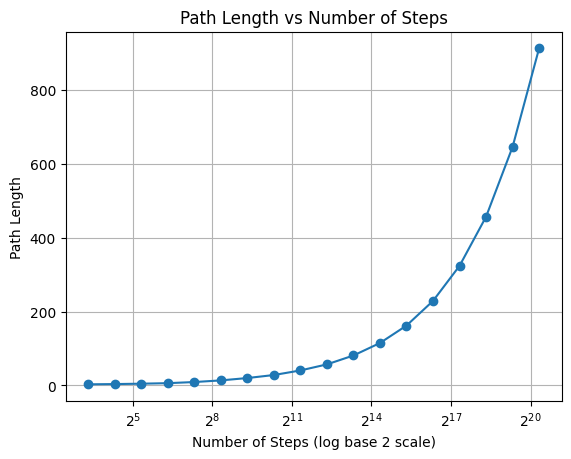
\includegraphics[width=0.75\linewidth]{path_length.png}
			\label{fig:placeholder}
		\end{figure}
		As the granularity of the steps increases, the total path length increases. This goes towards infinity as the number of steps increases. The time frame length for all of these paths is equal.
	\end{frame}

	\begin{frame}
	\centering 3. Variations of Brownian Motion
	\end{frame}

	% ---------------------------------------------------
	% 3.1 Absorbed Brownian Motion
	% ---------------------------------------------------
	\begin{frame}{3.1: Absorbed Brownian Motion}
		An absorbed Brownian motion behaves exactly like a standard Brownian motion until it hits a specific barrier $a$. Once it reaches $a$, the process is absorbed and remains fixed at that value forever.
		
		\vspace{0.5cm}
		\textbf{Definition:} Let $\tau_a = \inf\{t \ge 0 : W(t) = a\}$. The absorbed process $X(t)$ is:
		$$X(t) = \begin{cases}
			W(t) & \text{if } t < \tau_a \\
			a & \text{if } t \ge \tau_a,
		\end{cases}$$
		
	\end{frame}
	
	\begin{frame}{3.1: Absorbed Brownian Motion (Simulation)}
		\begin{figure}
			\centering
			\includegraphics[width=\textwidth]{"2_absorbed_brownian.png"}
			\caption{Paths and distribution of Absorbed Brownian Motion at barrier $a=0.5$}
		\end{figure}
	\end{frame}
	
	\begin{frame}{3.1: Derivation of Absorbed BM PDF}
		Let $W(t)$ be a standard Brownian motion and $a > 0$ be an absorbing barrier.
		The stopping time is
		$$\tau_a = \inf\{t > 0 : W(t) = a\}$$.
		
		For the absorbed process $X(t)$, we want to find the CDF for $x < a$:
		$$P(X(t) \le x) = P(W(t) \le x, \tau_a > t)$$
		
		Using the Law of Total Probability:
		$$P(W(t) \le x) = P(W(t) \le x, \tau_a > t) + P(W(t) \le x, \tau_a \le t)$$
		
		By symmetry, in standard brownian motion, paths can hit $x<a$ or $a+(a-x) = 2a-x$ at time $t \ge \tau_a$ with equal probability (going up or down the same amount has equal probability, this amount is $a-x$).
		$$P(W(t) \le x, \tau_a \le t) = P(W(t) \ge 2a - x, \tau_a \le t)$$
		
	\end{frame}
	
	\begin{frame}{3.1: Derivation of Absorbed BM PDF}
		Now observe that $W(t) > 2a-x$ implies $W(t) > a$ (since $x<a$). Thus, this means that $t \ge \tau_a$ and so the probability can be written as:
		$$P(W(t) \ge 2a - x, \tau_a \le t) = P(W(t) \ge 2a - x)$$
		
		Substituting the probability back into the CDF equation:
		$$P(X(t) \le x) = P(W(t) \le x) - P(W(t) \ge 2a - x)$$
		
		Using the standard normal CDF $\Phi$:
		$$F_{X(t)}(x) = \Phi\left(\frac{x}{\sqrt{t}}\right) - \left(1 - \Phi\left(\frac{2a - x}{\sqrt{t}}\right)\right)$$
		
		Since the normal distribution is symmetric, $1 - \Phi(z) = \Phi(-z)$:
		$$F_{X(t)}(x) = \Phi\left(\frac{x}{\sqrt{t}}\right) - \Phi\left(\frac{x - 2a}{\sqrt{t}}\right)$$
		
		Differentiating with respect to $x$ gives the PDF for $x < a$:
		$$f_{X(t)}(x) = \frac{1}{\sqrt{2\pi t}} \left( e^{-\frac{x^2}{2t}} - e^{-\frac{(x - 2a)^2}{2t}} \right)$$
	\end{frame}
	
	\begin{frame}{3.1: Hitting Time Probability in Standard BM}
		Now consider standard Brownian motion $W(t)$. The CDF of the hitting time $\tau_a$ is $P(\tau_a \le t)$.
		$$P(\tau_a \le t) = P(W(t) \ge a, \tau_a \le t) + P(W(t) < a, \tau_a \le t)$$
		
		By symmetry, $P(W(t) < a, \tau_a \le t) = P(W(t) \ge a, \tau_a \le t) = P(W(t) \ge a)$. Thus:
		$$P(\tau_a \le t) = 2P(W(t) \ge a) = 2 \left( 1 - \Phi\left(\frac{a}{\sqrt{t}}\right) \right)$$
		
		To find the probability of hitting $a$ in finite time, we take the limit as $t \to \infty$:
		$$\lim_{t \to \infty} P(\tau_a \le t) = 2 \left( 1 - \Phi(0) \right) = 2(1 - 0.5) = 1$$
		
		Therefore, standard Brownian motion hits any value $a$ in finite time with probability $1$.
	\end{frame}
	
	\begin{frame}{3.1: Expected Hitting Time is Infinite}
		To find the expected hitting time $\mathbb{E}[\tau_a]$, we first find the PDF of $\tau_a$ by differentiating its CDF with respect to $t$:
		$$f_{\tau_a}(t) = \frac{d}{dt} \left[ 2 \int_{a/\sqrt{t}}^{\infty} \frac{1}{\sqrt{2\pi}} e^{-\frac{z^2}{2}} dz \right] = \frac{a}{\sqrt{2\pi t^3}} e^{-\frac{a^2}{2t}}$$
		
		As $t \to \infty$, the integrand behaves like $t^{-1/2}$, which diverges (proof in next slide). Hence:
		$$\mathbb{E}[\tau_a] = \infty$$
		
		Because $P(\tau_a < \infty) = 1$ and $\mathbb{E}[\tau_a] = \infty$ for any arbitrary state $a$, every state in a standard Brownian motion is \textbf{null recurrent}.
	\end{frame}
	
	
	\begin{frame}{3.1: Expected Hitting Time is Infinite}
		The expected value is:
		\begin{align*}
			\mathbb{E}[\tau_a] &= \int_0^\infty P(\tau_a > t) \, dt \\
			&= \int_0^\infty \left( 1 - \frac{2}{\sqrt{2\pi}} \int_{a/\sqrt{t}}^\infty e^{-y^2/2} \, dy \right) dt \\
			&= \frac{2}{\sqrt{2\pi}} \int_0^\infty \int_0^{a/\sqrt{t}} e^{-y^2/2} \, dy \, dt \\
			&= \frac{2}{\sqrt{2\pi}} \int_0^\infty \int_0^{a^2/y^2} dt \, e^{-y^2/2} \, dy \\
			&= \frac{2a^2}{\sqrt{2\pi}} \int_0^\infty \frac{1}{y^2} e^{-y^2/2} \, dy \\
			&\ge \frac{2a^2 e^{-1/2}}{\sqrt{2\pi}} \int_0^1 \frac{1}{y^2} \, dy \\
			&= \infty.
		\end{align*}
	\end{frame}
	
	% ---------------------------------------------------
	% 3.2 Reflected Brownian Motion
	% ---------------------------------------------------
	\begin{frame}{3.2: Reflected Brownian Motion at Origin}
		Reflected Brownian motion behaves like a standard Brownian motion but is constrained to be non-negative. Whenever the process hits $0$, it bounces back into the positive domain.
		
		\vspace{0.5cm}
		\textbf{Definition:} The standard reflected Brownian motion is the absolute value of a standard Brownian motion:
		$$Z(t) = |W(t)|$$
	\end{frame}
	
	\begin{frame}{3.2: Reflected Brownian Motion (Simulation)}
		\begin{figure}
			\centering
			\includegraphics[width=\textwidth]{"3_reflected_brownian.png"}
			\caption{Paths and distribution of Reflected Brownian Motion}
		\end{figure}
	\end{frame}
	
	\begin{frame}{3.2: Distribution of Reflected Brownian Motion}		
		The distribution of $Z(t)$ is obtained as:
		
		For $y > 0$,
		\begin{align*}
			P(Z(t) \le y) &= P(-y \le W(t) \le y) \\
			&= P(W(t) \le y) - P(W(t) \le -y) \\
			&= 2P(W(t) \le y) - 1 \\
			&= \frac{2}{\sqrt{2\pi t}} \int_{-\infty}^{y} e^{-x^2 / 2t} \, dx - 1,
		\end{align*}
		($P(W(t) \le -y) = 1-P(W(t) \le y)$, due to W(t) having gaussian distribution)
		
		\begin{itemize}
			\item Expected value: $ \mathbb{E}[Z(t)] = \sqrt{\frac{2t}{\pi}} $
			\item Variance: $ \text{Var}(Z(t)) = \left( 1 - \frac{2}{\pi} \right) t $
		\end{itemize}
		
	\end{frame}
	
	% ---------------------------------------------------
	% 3.3 Geometric Brownian Motion
	% ---------------------------------------------------
	\begin{frame}{3.3: Geometric Brownian Motion}
		If $\{W(t), t \ge 0\}$ is a standard Brownian motion, then the process $\{Y(t), t \ge 0\}$, defined by
		$$Y(t) = e^{W(t)}, \quad t \ge 0,$$
		is called \textbf{geometric Brownian motion}.
	\end{frame}
	
	\begin{frame}{3.3: Geometric Brownian Motion (Simulation)}
		\begin{figure}
			\centering
			\includegraphics[width=\textwidth]{"4_geometric_brownian.png"}
			\caption{Paths and Log-Normal distribution of GBM}
		\end{figure}
	\end{frame}
	
	\begin{frame}{3.3: Geometric Brownian Motion: Definition and Moments}
		Since $W(t)$ is normal with mean $0$ and variance $t$, its MGF is given by:
		$$\mathbb{E}[e^{sW(t)}] = e^{ts^2/2}$$
		
		Using this, we can compute the mean and variance of Y(t):
		\begin{align*}
			\mathbb{E}[Y(t)] &= \mathbb{E}[e^{W(t)}] = e^{t/2} \\
			\text{Var}(Y(t)) &= \mathbb{E}[Y^2(t)] - (\mathbb{E}[Y(t)])^2 \\
			&= \mathbb{E}[e^{2W(t)}] - e^t \\
			&= e^{2t} - e^t.
		\end{align*}
	\end{frame}
		
	\begin{frame}{3.3: GBM Example: Modelling stock prices}
		Using discrete real-world observations and assumptions (like stock prices):
		\begin{itemize}
			\item Let $Y(n)$ be a stock price at day $n$.
			\item Assume the daily \textbf{percentage returns}, $X_i = \frac{Y(i)}{Y(i-1)}$, are i.i.d.
		\end{itemize}
		
		\vspace{0.3cm}
		The price at time $n$ is the product of all previous returns:
		$$Y(n) = Y(0) X_1 X_2 \cdots X_n$$
		
		Taking the logarithm turns the product into a sum of i.i.d. variables:
		$$\log Y(n) = \log Y(0) + \sum_{i=1}^n \log X_i$$
		
		\vspace{0.3cm}
		By the \textbf{Central Limit Theorem}, this sum of i.i.d. variables converges to a Brownian motion as the time steps become continuous. Thus, $Y(t)$ naturally becomes a Geometric Brownian Motion.
	\end{frame}
	
	\begin{frame}{3.3: Discrete Prices and Multiplicative Returns}
		Before jumping to continuous calculus, we observe real-world markets in discrete time steps (e.g., daily closing prices).
		
		\begin{itemize}
			\item Let $Y(n)$ be the price of an asset at day $n$.
			\item Let $X_i = \frac{Y(i)}{Y(i-1)}$ be the gross return on day $i$. 
			\item We assume these daily returns $X_i$ are \textbf{independent and identically distributed (i.i.d.)}.
		\end{itemize}
		
		The price at day $n$ is simply the initial price multiplied by all subsequent daily returns:
		$$Y(n) = Y(0) X_1 X_2 \cdots X_n$$
	\end{frame}
	
	\begin{frame}{3.3: Discrete Prices and Multiplicative Returns}
		Taking the natural logarithm transforms the product into a sum:
		$$\log Y(n) = \log Y(0) + \sum_{i=1}^n \log X_i$$
		
		\begin{itemize}
			\item Let $Z_i = \log X_i$. Since the $X_i$ are i.i.d., the $Z_i$ terms are also i.i.d.
			\item Let the mean be $\mathbb{E}[Z_i] = \mu$ and variance be $\text{Var}(Z_i) = \sigma^2$.
			\item We define our sum: $S_n = \sum_{i=1}^n Z_i$.
		\end{itemize}
		
		The Central Limit Theorem (CLT) applies to our sum $S_n$, by appropriate scaling.
		
		Subtract its mean ($n\mu$) and divide by its standard deviation ($\sigma\sqrt{n}$):
		
		\begin{equation*}
			\frac{S_n - n\mu}{\sigma \sqrt{n}} \xrightarrow{d} \mathcal{N}(0, 1) \quad \text{as } n \to \infty
		\end{equation*}
		
		Thus $S_n$ becomes a gaussian random variable with mean $n\mu$ and variance $n\sigma^2$.
		$$S_n \sim \mathcal{N}(n\mu, n\sigma^2)$$
	\end{frame}

	% ---------------------------------------------------
	% 3.4 Integrated Brownian Motion
	% ---------------------------------------------------
	\begin{frame}{3.4: Integrated Brownian Motion}
		If $\{W(t), t \ge 0\}$ is a standard Brownian motion, the \textbf{integrated Brownian motion} $\{Y(t), t \ge 0\}$ is defined as the area under the Brownian path:
		$$Y(t) = \int_0^t W(s) \, ds$$
		
		\textbf{Physical Intuition:}
		\begin{itemize}
			\item If $W(t)$ represents the random \textit{velocity} of a particle subject to continuous random shocks...
			\item ...then $Y(t)$ represents the \textit{position} of that particle.
		\end{itemize}
		
		\textbf{Smoothness:} While $W(t)$ is jagged and nowhere differentiable, integration is a smoothing operation. $Y(t)$ is continuously differentiable, and its derivative is exactly $\frac{d}{dt}Y(t) = W(t)$. The path for IBM is smooth.
	\end{frame}
	
	\begin{frame}{3.4: Integrated Brownian Motion (Simulation)}
		\begin{figure}
			\centering
			\includegraphics[width=\textwidth]{"5_integrated_brownian.png"}
			\caption{Paths and distribution of Integrated Brownian Motion}
		\end{figure}
	\end{frame}
	
	\begin{frame}{3.4: Y(t) is Gaussian}
		The variables of a Brownian motion at any finite set of times are \textbf{jointly Gaussian}.
		
		\vspace{0.3cm}
		Consider any sequence of times $0 < t_1 < t_2 < \dots < t_n$. By the definition of Brownian motion, the \textit{increments} are independent and normally distributed:
		\begin{align*}
			Z_1 &= W(t_1) - W(0) \sim \mathcal{N}(0, t_1) \\
			Z_2 &= W(t_2) - W(t_1) \sim \mathcal{N}(0, t_2 - t_1) \\
			&\vdots \\
			Z_n &= W(t_n) - W(t_{n-1}) \sim \mathcal{N}(0, t_n - t_{n-1})
		\end{align*}
		
		Because the increments $Z_i$ are independent Gaussians, the vector $\mathbf{Z} = [Z_1, Z_2, \dots, Z_n]^T$ is trivially a \textbf{jointly Gaussian vector}.
	\end{frame}
	
	\begin{frame}{3.4: Y(t) is Gaussian}
		We can express the actual Brownian motion values $W(t_k)$ as a cumulative sum of these independent Gaussian increments:
		\begin{align*}
			W(t_1) &= Z_1 \\
			W(t_2) &= Z_1 + Z_2 \\
			&\vdots \\
			W(t_n) &= Z_1 + Z_2 + \dots + Z_n
		\end{align*}
		
		\vspace{0.3cm}
		\textbf{Property:} Any linear transformation of a jointly Gaussian vector results in another jointly Gaussian vector. 
		
		\vspace{0.3cm}
		Since $\mathbf{W} = [W(t_1), \dots, W(t_n)]^T$ is just a linear combination of $\mathbf{Z}$, we conclude that \textbf{$W(t)$ at any set of time instants is jointly Gaussian}.
	\end{frame}
	
	\begin{frame}{3.4: Y(t) is Gaussian}		
		Using the definition of Riemann integral as a limit of sums over small time steps $\Delta s$:
		$$Y(t) \approx \sum_{i=1}^n W(s_i) \Delta s$$
		
		\begin{itemize}
			\item From our previous proof, the variables $(W(s_1), W(s_2), \dots, W(s_n))$ are jointly Gaussian.
			\item A finite linear combination of jointly Gaussian variables is strictly Gaussian.
			\item The limit of a sequence of Gaussian random variables (as $\Delta s \to 0$) is also Gaussian.
		\end{itemize}
		
		Therefore, $Y(t)$ is a normally distributed random variable. We just need its parameters.
	\end{frame}
	
	\begin{frame}{3.4: Parameters of IBM: Expected Value}
		Since integration is a linear operator, we can pass the expectation directly inside the integral, indirectly applying linearity of expectation to variables in the Riemann integral
		
		The mean of the integrated Brownian motion is:
		\begin{align*}
			\mathbb{E}[Y(t)] &= \mathbb{E}\left[ \int_0^t W(s) \, ds \right] \\
			&= \int_0^t \mathbb{E}[W(s)] \, ds
		\end{align*}
		
		Because standard Brownian motion has a mean of zero at all times ($\mathbb{E}[W(s)] = 0$):
		$$ \mathbb{E}[Y(t)] = \int_0^t 0 \, ds = 0 $$
	\end{frame}
	
	\begin{frame}{3.4: Parameters of IBM: Variance}
		To find the variance, we calculate $\mathbb{E}[Y(t)^2]$ since the mean is zero. We square the integral by writing it as a double integral with dummy variables $u$ and $v$:
		
		\begin{align*}
			\text{Var}(Y(t)) &= \mathbb{E}\left[ \left( \int_0^t W(s) \, ds \right)^2 \right] \\
			&= \mathbb{E}\left[ \int_0^t W(u) \, du \int_0^t W(v) \, dv \right] \\
			&= \mathbb{E}\left[ \int_0^t \int_0^t W(u)W(v) \, du \, dv \right]
		\end{align*}
		
		\vspace{0.3cm}
		Passing the expectation inside the double integral:
		$$ \text{Var}(Y(t)) = \int_0^t \int_0^t \mathbb{E}[W(u)W(v)] \, du \, dv $$
	\end{frame}
	
	\begin{frame}{3.4: Covariance of Standard Brownian Motion}
		To evaluate the double integral for the variance, we need the covariance of standard Brownian motion: $\mathbb{E}[W(u)W(v)]$. Let's derive it.
		
		\vspace{0.3cm}
		Assume without loss of generality that $u \le v$. We can rewrite the value of the Brownian motion at the later time $v$ as its value at the earlier time $u$ plus the increment that occurred between $u$ and $v$:
		$$ W(v) = W(u) + (W(v) - W(u)) $$
		
		\vspace{0.3cm}
		Substitute this expanded form of $W(v)$ into the expectation:
		\begin{align*}
			\mathbb{E}[W(u)W(v)] &= \mathbb{E}\big[W(u) \cdot \big(W(u) + W(v) - W(u)\big)\big] \\
			&= \mathbb{E}\big[W(u)^2 + W(u)(W(v) - W(u))\big]
		\end{align*}
	\end{frame}
	
	\begin{frame}{3.4: Covariance of Standard Brownian Motion}
		Using the linearity of expectation, we split the expression into two terms, and using W(0) = 0:
		$$ \mathbb{E}[W(u)W(v)] = \mathbb{E}[W(u)^2] + \mathbb{E}[(W(u) - W(0))(W(v) - W(u))] $$
		
		\vspace{0.3cm}
		Now, we analyze the two terms:
		\begin{enumerate}
			\item \textbf{First Term:} Since $W(u) \sim \mathcal{N}(0, u)$, its second moment (which is its variance) is exactly $\mathbb{E}[W(u)^2] = u$.
			\item \textbf{Second Term:} Because Brownian motion has \textit{independent increments}, the increment $W(u) - W(0)$ is independent of the non overlapping future increment $W(v) - W(u)$. Thus:
			$$ \mathbb{E}[W(u) - W(0)] \cdot \mathbb{E}[W(v) - W(u)] = 0 \cdot 0 = 0 $$
		\end{enumerate}
		
		\vspace{0.3cm}
		Adding them yields $\mathbb{E}[W(u)W(v)] = u + 0 = u$. Similarly, if $v \le u$ instead, the result would be $v$. Therefore, the covariance is always $\min(u, v)$.
	\end{frame}
	
	\begin{frame}{3.4: Parameters of IBM: Covariance}
		Since $\{Y(t), t \ge 0\}$ is a Gaussian process, its distribution is fully characterized by its mean value and covariance function. 
		
		\vspace{0.3cm}
		For $s \le t$, we compute the covariance:
		\begin{align*}
			\text{Cov}[Y(s), Y(t)] &= \mathbb{E}[Y(s)Y(t)] \\
			&= \mathbb{E}\left[ \int_0^s W(y) \, dy \int_0^t W(u) \, du \right] \\
			&= \int_0^s \int_0^t \mathbb{E}[W(y)W(u)] \, du \, dy \\
			&= \int_0^s \int_0^t \min(y, u) \, du \, dy
		\end{align*}
	\end{frame}
	
	\begin{frame}{3.4: Parameters of IBM: Covariance}
		To evaluate $\int_0^s \int_0^t \min(y, u) \, du \, dy$ for $s \le t$, we split the inner integral at $u=y$:
		
		\begin{align*}
			\text{Cov}[Y(s), Y(t)] &= \int_0^s \left( \int_0^y u \, du + \int_y^t y \, du \right) dy \\
			&= \int_0^s \left( \frac{y^2}{2} + y(t - y) \right) dy \\
			&= \int_0^s \left( yt - \frac{y^2}{2} \right) dy \\
			&= t\frac{s^2}{2} - \frac{s^3}{6} \\
			&= s^2 \left( \frac{t}{2} - \frac{s}{6} \right)
		\end{align*}
		
		\vspace{0.2cm}
		\textit{Note: Setting $s=t$ immediately recovers the variance $t^3/3$.}
		
		\vspace{0.2cm}
		\textbf{Conclusion:} For any time $t$, $Y(t) \sim \mathcal{N}\left(0, \frac{t^3}{3}\right)$.
	\end{frame}
	
	\begin{frame}{3.4: Markov Process (Y(t), W(t))}
		While $Y(t)$ alone is not a Markov process, the vector process $\{(Y(t), W(t)), t \ge 0\}$ is Markov. Because they are jointly normal, their joint distribution is defined by their cross-covariance.
		
		\vspace{0.2cm}
		We analyze the difference over a small step $h$:
		\begin{align*}
			\text{Cov}(Y(t), Y(t) - Y(t-h)) &= \text{Cov}(Y(t), Y(t)) - \text{Cov}(Y(t), Y(t-h)) \\
			&= \frac{t^3}{3} - (t-h)^2 \left[ \frac{t}{2} - \frac{t-h}{6} \right] \\
			&= \frac{t^2h}{2} + o(h)
		\end{align*}
		
		\vspace{0.2cm}
		Alternatively, expressing the difference as an integral:
		\begin{align*}
			\text{Cov}(Y(t), Y(t) - Y(t-h)) &= \text{Cov}\left(Y(t), \int_{t-h}^t W(s) \, ds\right) \\
			&= \text{Cov}(Y(t), hW(t) + o(h)) \\
			&= h\text{Cov}(Y(t), W(t)) + o(h)
		\end{align*}
	\end{frame}
	
	\begin{frame}{3.4: The Bivariate Normal Distribution}
		Equating the two expressions for the covariance over step $h$:
		$$h\text{Cov}(Y(t), W(t)) \approx \frac{t^2h}{2}$$
		
		\vspace{0.3cm}
		Dividing by $h$ and taking the limit as $h \to 0$ gives the cross-covariance:
		$$\text{Cov}(Y(t), W(t)) = \frac{t^2}{2}$$
		
		\vspace{0.3cm}
		Hence, the joint state of the integrated process and the Brownian motion, $(Y(t), W(t))$, has a bivariate normal distribution with:
		\begin{align*}
			\mathbb{E}[Y(t)] &= \mathbb{E}[W(t)] = 0 \\
			\text{Var}(Y(t)) &= \frac{t^3}{3}, \quad \text{Var}(W(t)) = t \\
			\text{Cov}(Y(t), W(t)) &= \frac{t^2}{2}
		\end{align*}
	\end{frame}
	
	\begin{frame}{3.4: Exponential Integrated Brownian Motion}
		Another form of integrated Brownian motion arises if we assume the \textit{percent rate of change} of a price follows a Brownian motion process (similar to what we did in GBM).
		
		If $P(t)$ denotes the price at time $t$, then:
		$$\frac{d}{dt} P(t) = W(t)P(t)$$
		
		Solving this differential equation yields:
		$$P(t) = P(0) \exp\left\{ \int_0^t W(s) \, ds \right\} = P(0) e^{Y(t)}$$
		
		Taking $P(0) = 1$, we have $P(t) = e^{Y(t)}$. Since $Y(t)$ is normal with mean 0 and variance $t^3/3$, $P(t)$ is log-normally distributed.
		
		$$\mathbb{E}[P(t)] = \mathbb{E}\left[e^{Y(t)}\right] = \exp\left\{ \frac{t^3}{6} \right\}$$
		
		The above comes from the $M_Y(1)$ where $M_Y$ is the MGF of $Y(t)$.
	\end{frame}
	
	% ---------------------------------------------------
	% 3.5 Brownian Motion with Drift
	% ---------------------------------------------------
	\begin{frame}{3.5: Brownian Motion with Drift}
		A Brownian motion with drift represents a standard Brownian motion that is shifted by a constant trend over time.
		
		\vspace{0.5cm}
		\textbf{Definition:} The process $X(t)$ is defined as:
		$$X(t) = \mu t + \sigma W(t)$$
		
		\vspace{0.2cm}
		Where $\mu$ is the constant drift rate and $\sigma$ is the volatility. At time $t$, $X(t)$ is normally distributed with mean $\mu t$ and variance $\sigma^2 t$.
	\end{frame}
	
	\begin{frame}{3.5: Brownian Motion with Drift (Simulation)}
		\begin{figure}
			\centering
			\includegraphics[width=\textwidth]{"6_drift_brownian.png"}
			\caption{Paths and distribution of Brownian Motion with Drift}
		\end{figure}
	\end{frame}
	
	% ---------------------------------------------------
	% Slide 1: Problem Setup
	% ---------------------------------------------------
	\begin{frame}{3.5: Optimal Stopping Time}
		Let $X(t)$ be a Brownian motion with drift $\mu$ and variance $\sigma^2t$.
		
		\vspace{0.3cm}
		We want to compute the probability that the process hits an upper barrier $A > 0$ before a lower barrier $-B < 0$.
		
		\vspace{0.3cm}
		Let $P(x)$ denote this probability, conditioned on starting at a position $x \in (-B, A)$. So $X(0)$ need not be 0:
		$$P(x) = P(X(t) \text{ hits } A \text{ before } -B \mid X(0) = x)$$
		
		\vspace{0.3cm}
		To find $P(x)$, we will observe the process over a microscopic time interval $[0, h]$. Let $Y = X(h) - X(0)$ be the random step taken during this time.
	\end{frame}
	
	% ---------------------------------------------------
	% Slide 2: The Law of Total Probability
	% ---------------------------------------------------
	\begin{frame}{3.5: Optimal Stopping Time}
		Let $H$ be the event that the process hits either barrier ($A$ or $-B$) during the microscopic time interval $[0, h]$. Let Win be the event that the process hits $A$ before it hits $-B$.
		
		\vspace{0.3cm}
		By the Law of Total Probability, we can split $P(x)$ into two scenarios:
		\begin{align*}
			P(x) &= P(\text{Win} \mid H) P(H) \\
			&+ P(\text{Win} \mid H^c) P(H^c)
		\end{align*}
		
		\vspace{0.3cm}
		Because Brownian paths are continuous and $x$ is strictly inside $(-B, A)$, moving a macroscopic distance to a boundary in a infinitesimal time $h$ is small.
		
		\vspace{0.3cm}
		Mathematically, $P(H)$ shrinks to zero faster than $h$, so $P(H) = o(h)$.
	\end{frame}
	
	% ---------------------------------------------------
	% Slide 3: Isolating the Relevant Scenario
	% ---------------------------------------------------
	\begin{frame}{3.5: Optimal Stopping Time}
		Using $P(H) = o(h)$,
		\begin{align*}
			P(x) &= P(\text{Win} \mid H) \cdot o(h) + P(\text{Win} \mid H^c) (1 - o(h)) \\
			P(x) &= P(\text{Win} \mid H^c) + o(h)
		\end{align*}
		\textit{(Note that $o(h) \times bounded = o(h)$, here the difference of probabilities is bounded between $-1$ and $1$)}
		
		\vspace{0.3cm}
		This tells us that for an infinitesimally small step $h$, we can safely assume the process has not yet hit a boundary. 
		
	\end{frame}
	
	% ---------------------------------------------------
	% Slide 4: The Markov Property and Expectation
	% ---------------------------------------------------
	\begin{frame}{3.5: Optimal Stopping Time}
		Markov property dictates that the future evolution of the process is dependent only on the present:
		$$ \mathbb{P}(\text{Future} \mid \text{Present}, \text{Past}) = \mathbb{P}(\text{Future} \mid \text{Present}) $$
		$$ \mathbb{P}(W \mid X(h) = x+Y, H^C, X(0) = x) = \mathbb{P}(W \mid X(h) = x+Y) $$
		
		Because Brownian motion is \textbf{time-homogeneous}, the probability of winning starting from position $x+Y$ at time $h$ is identical to starting there at time $0$:
		$$ \mathbb{P}(W \mid X(h) = x+Y) = P(x+Y) $$
		
		Integrating over all possible values $Y=y$ of the random step $Y = X(h) - X(0)$ yields the total expectation: $\mathbb{E}[P(x+Y)]$.
	\end{frame}
	
	% ---------------------------------------------------
	% Slide 5: Taylor Series Expansion
	% ---------------------------------------------------
	\begin{frame}{3.5: Optimal Stopping Time}
		We now proceed by taking a Taylor series expansion of $P(x + Y)$ about $x$:
		$$P(x+Y) = P(x) + P'(x)Y + \frac{P''(x)}{2}Y^2 + \cdots$$
		
		\vspace{0.3cm}
		Substitute this expansion into our expectation equation:
		$$P(x) = \mathbb{E}\left[P(x) + P'(x)Y + \frac{P''(x)}{2}Y^2\right] + o(h)$$
		
		\vspace{0.3cm}
		Since $Y \sim \mathcal{N}(\mu h, h)$, we know its moments:
		\begin{itemize}
			\item $\mathbb{E}[Y] = \mu h$
			\item $\mathbb{E}[Y^2] = \text{Var}(Y) + (\mathbb{E}[Y])^2 = \sigma^2h + \mu^2 h^2 = h + o(h)$
		\end{itemize}
		\textit{(Higher-order terms like $Y^3$ yield expectations that are $o(h)$).}
	\end{frame}
	
	% ---------------------------------------------------
	% Slide 6: Forming the Differential Equation
	% ---------------------------------------------------
	\begin{frame}{3.5: Optimal Stopping Time}
		Applying the expectations to our expansion:
		$$P(x) = P(x) + P'(x)\mu h + \frac{P''(x)}{2}\sigma^2h + o(h)$$
		
		\vspace{0.3cm}
		Subtract $P(x)$ from both sides, divide the entire equation by $h$, and isolate the terms:
		$$P'(x)\mu + \frac{P''(x)}{2}\sigma^2 = \frac{o(h)}{h}$$
		
		\vspace{0.3cm}
		Letting the time step $h \to 0$, the $\frac{o(h)}{h}$ term vanishes by definition. This leaves us with a second-order linear differential equation:
		$$P'(x)\mu + \frac{P''(x)}{2}\sigma^2 = 0$$
	\end{frame}
	
	% ---------------------------------------------------
	% Slide 7: Solving the Differential Equation
	% ---------------------------------------------------
	\begin{frame}{3.5: Optimal Stopping Time}
		Integrating once yields $e^{2(\mu/\sigma^2) x} P'(x) = c_1$. 
		Integrating a second time gives the general solution:
		$$P(x) = C_1 + C_2 e^{-2(\mu/\sigma^2) x}$$
		
		We use the boundary conditions $P(A) = 1$ and $P(-B) = 0$ to solve for $C_1$ and $C_2$:
		\begin{align*}
			C_1 + C_2 e^{-2(\mu/\sigma^2) A} &= 1 \\
			C_1 + C_2 e^{2(\mu/\sigma^2) B} &= 0
		\end{align*}
		
		\vspace{0.2cm}
		Solving this linear system yields:
		$$C_1 = \frac{e^{2(\mu/\sigma^2) B}}{e^{2(\mu/\sigma^2) B} - e^{-2(\mu/\sigma^2) A}}, \quad C_2 = \frac{-1}{e^{2(\mu/\sigma^2) B} - e^{-2(\mu/\sigma^2) A}}$$
		
		\vspace{0.2cm}
		Substituting $C_1$ and $C_2$ back gives the probability from any starting point $x$:
		$$P(x) = \frac{e^{2(\mu/\sigma^2) B} - e^{-2(\mu/\sigma^2) x}}{e^{2(\mu/\sigma^2) B} - e^{-2(\mu/\sigma^2) A}}$$
	\end{frame}
%------------------------------------------------
%------------------------------------------------
%------------------------------------------------
%------------------------------------------------%------------------------------------------------
%------------------------------------------------%------------------------------------------------%------------------------------------------------%------------------------------------------------%------------------------------------------------%------------------------------------------------%------------------------------------------------%------------------------------------------------%------------------------------------------------%------------------------------------------------%------------------------------------------------%------------------------------------------------%------------------------------------------------%------------------------------------------------%------------------------------------------------%------------------------------------------------%------------------------------------------------%------------------------------------------------%------------------------------------------------%------------------------------------------------%------------------------------------------------%------------------------------------------------%------------------------------------------------%------------------------------------------------%------------------------------------------------%------------------------------------------------%------------------------------------------------%------------------------------------------------%------------------------------------------------%------------------------------------------------%------------------------------------------------%------------------------------------------------
	\begin{frame}
	\centering 4. Diffusion Equations, Intro to Stochastic Calculus
	\end{frame}

	%------------------------------------------------
\begin{frame}
\begin{beamercolorbox}[wd=\paperwidth,sep=0.3cm,center]{frametitle}
\usebeamerfont{frametitle}Backward Diffusion Equation
\end{beamercolorbox}
\end{frame}
%------------------------------------------------
%------------------------------------------------
\begin{frame}{Motivation}
We want the density of the random variable $X(t)$. The backward approach conditions on the value of $X(h)$—that is, it looks all the way back to the process at time $h$. The forward approach conditions on $X(t - h)$.

\vspace{0.3cm}
\textbf{Formal Definitions:}
\begin{itemize}
    \item $X(t)$: A continuous-time stochastic process (such as a Brownian motion process with drift coefficient $\mu$) representing the state of the random variable at time $t$.
    \item $p(x, t, y)$: The transition probability density function. It denotes the probability density of $X(t)$ being in state $x$, given the initial condition $X(0) = y$.
\end{itemize}

\vspace{0.3cm}
Mathematically, this is defined as:
$$p(x, t, y) = \lim_{\Delta x \to 0} \frac{P\{x < X(t) < x + \Delta x \mid X(0) = y\}}{\Delta x}$$
\end{frame}

%------------------------------------------------
%------------------------------------------------
\begin{frame}{Backward Approach}

\textbf{Conditioning on the First Step} \\
The backward approach fundamentally conditions on the value of the process at a small time step $h$, denoted as $X(h)$. We are analyzing the outcome of the very first random step out of the starting state $y$.

\vspace{0.3cm}


\textbf{Law of Total Probability \& The Markov Property} \\
To find the probability density of reaching $x$ at time $t$, we condition on all possible intermediate states $z$ at time $h$. 

Because the process is Markovian, its future depends only on its present state. Therefore, the probability of reaching state $x$ at time $t$, given that it was at state $z$ at time $h$, is equivalent to starting at $z$ and reaching $x$ in the remaining time $t - h$.

\end{frame}

% %------------------------------------------------
% \begin{frame}{Explanation}
% Here, we took a subtle leap of faith, and directly equated
% $p(x, t, y)$ with the expectation.

% Let's go step by step.

% After defining $p(x, t, y)$ as the probability density of $X(t)$ given $X(0) = y$, we use the LAW OF TOTAL PROBABILITY and the MARKOVIAN PROPERTY to write:
% \end{frame}

% %------------------------------------------------
%------------------------------------------------
\begin{frame}{The Chapman-Kolmogorov Foundation}

\begin{block}{Transition Probability Density}
\begin{itemize}
    \item Let $p(x, t \mid y, 0)$ be the transition probability density of moving from state $y$ at time $0$ to state $x$ at time $t$.
    \item For \textbf{time-homogeneous processes}, we write this as $p(x, t \mid y)$.
\end{itemize}
\end{block}

\vspace{0.2cm}

\begin{block}{The Core Equation}
The Chapman-Kolmogorov equation states that to go from $y$ to $x$ in time $t$, we must integrate over all possible \textbf{intermediate states} $z$ at some intermediate time $h$:



$$p(x, t \mid y) = \int_{-\infty}^{\infty} p(x, t - h \mid z) p(z, h \mid y) dz$$
\end{block}

\end{frame}

%------------------------------------------------
%------------------------------------------------
\begin{frame}{The Change of Variables (Defining the Jump)}

\vspace{-0.4cm}

\textbf{The Random Displacement:}
\begin{itemize}
    \item To evaluate how the state changes over the small time interval $h$, we define the random displacement (the jump) as $\Delta y = z - y$. 
    \item Consequently, the intermediate state can be expressed as $z = y + \Delta y$.
\end{itemize}

\vspace{0.3cm}

The term $p(z, h \mid y) dz$ represents the probability of the process moving from $y$ to $z$ in time $h$. 

\vspace{0.3cm}

The unconditional increment $X(t+h) - X(t)$ has a \textbf{Normal Distribution} that depends only on the time step $h$.
The probability of making a jump of size $\Delta y$ is thus identical no matter where you are on the real line.

\end{frame}
\begin{frame}

The density of the jump $\Delta y$ is simply the Gaussian PDF of $\mathcal{N}(\mu h, $\sigma^2$h$)$ by definition of Brownian Motion. 

\vspace{0.8cm}
\textbf{The Rewritten Integral:}
Because of this spatial homogeneity, we can rigorously denote the probability density of this specific jump as $f_h(\Delta y) \equiv p(y + \Delta y, h \mid y)$. 
\vspace{0.5cm}

Substituting $z = y + \Delta y$ and $dz = d(\Delta y)$, we rewrite the Chapman-Kolmogorov integral as:
$$p(x, t \mid y) = \int_{-\infty}^{\infty} p(x, t - h \mid y + \Delta y) f_h(\Delta y) d(\Delta y)$$

\end{frame}

%------------------------------------------------
\begin{frame}{Taylor Expansion}

Now we apply a formal Taylor expansion to the deterministic function $p(x, t - h | y + \Delta y)$. We expand around the point $(t, y)$, taking a step of $-h$ in the time dimension and $\Delta y$ in the space dimension.

The function we are expanding is $p(x, t|y)$, which maps a 3-tuple input to a scalar output.

\begin{itemize}
\item Our \textbf{anchor point} of evaluation is $(x, t, y)$.
\item Our \textbf{perturbed point} is $(x, t - h, y + \Delta y)$.
\item Our \textbf{displacement vector} is therefore $(0, -h, \Delta y)$.
\end{itemize}

Because the displacement in the $x$-dimension is exactly $0$, all partial derivatives involving $x$ vanish immediately. This leaves us with only the active terms involving $t$ and $y$.

\end{frame}

%------------------------------------------------
\begin{frame}{General Taylor Expansion}

Here is the detailed Taylor series expansion for a scalar-valued function of three variables, $f : \mathbb{R}^3 \rightarrow \mathbb{R}$.
\vspace{-0.3cm}
\begin{align*}
f(x, y, z) &= f(x_0, y_0, z_0) \\
&\quad + \left( \frac{\partial f}{\partial x} \Delta x + \frac{\partial f}{\partial y} \Delta y + \frac{\partial f}{\partial z} \Delta z \right) \\
&\quad + \frac{1}{2!} \left( \frac{\partial^2 f}{\partial x^2} (\Delta x)^2 + \frac{\partial^2 f}{\partial y^2} (\Delta y)^2 + \frac{\partial^2 f}{\partial z^2} (\Delta z)^2 \right. \\
&\quad \left. + 2\frac{\partial^2 f}{\partial x \partial y} \Delta x \Delta y + 2\frac{\partial^2 f}{\partial x \partial z} \Delta x \Delta z + 2\frac{\partial^2 f}{\partial y \partial z} \Delta y \Delta z \right) \\
&\quad + \mathcal{O}(||\Delta \mathbf{x}||^3)
\end{align*}

If we want to expand a continuously differentiable function $f(x, y, z)$ around a specific point $(x_0, y_0, z_0)$, we can express the coordinates of a nearby point as $x = x_0 + \Delta x$, $y = y_0 + \Delta y$, and $z = z_0 + \Delta z$.
\end{frame}
%------------------------------------------------
% \begin{frame}{Clairaut's Theorem}

% (Note: All partial derivatives are evaluated at the expansion point $(x_0, y_0, z_0)$, and by Clairaut's theorem, we assume the mixed partial derivatives are equal, e.g., $\frac{\partial^2 f}{\partial x \partial y} = \frac{\partial^2 f}{\partial y \partial x}$.)

% (when is clariut's theorem not true?)
% \end{frame}

%------------------------------------------------
%------------------------------------------------
%------------------------------------------------
\begin{frame}{Taylor Expansion of Transition Density}

Expanding $p(x, t - h \mid y + \Delta y)$ around the anchor point $(x, t, y)$ using the multi-variable Taylor series:

\begin{align*}
&p(x, t - h \mid y + \Delta y) = p(x, t \mid y) + \left( -h \frac{\partial p}{\partial t} + \Delta y \frac{\partial p}{\partial y} \right) \\
&+ \frac{1}{2!} \left( (-h)^2 \frac{\partial^2 p}{\partial t^2} + 2(-h)(\Delta y) \frac{\partial^2 p}{\partial t \partial y} + (\Delta y)^2 \frac{\partial^2 p}{\partial y^2} \right) + \mathcal{O}(h^3, (\Delta y)^3)
\end{align*}

We then group the higher-order terms, as well as the $(-h)^2$ and cross-derivative terms—which will vanish faster than $h$ in the limit as $h \to 0$—into a remainder function, $G(h, \Delta y)$:

$$p(x, t - h \mid y + \Delta y) = p(x, t \mid y) - h \frac{\partial p}{\partial t} + \Delta y \frac{\partial p}{\partial y} + \frac{1}{2} (\Delta y)^2 \frac{\partial^2 p}{\partial y^2} + G(h, \Delta y)$$

\end{frame}

%------------------------------------------------
%------------------------------------------------
\begin{frame}{Substitute into Chapman-Kolmogorov}

Substitute the rigorous expansion back into the Chapman-Kolmogorov integral:

$$p(x, t \mid y) = \int_{-\infty}^{\infty} \left[ p(x, t \mid y) - h \frac{\partial p}{\partial t} + \Delta y \frac{\partial p}{\partial y} + \frac{1}{2} (\Delta y)^2 \frac{\partial^2 p}{\partial y^2} + 

\hfill \left.G(h, \Delta y) \right] f_h(\Delta y) d(\Delta y)$$

\vspace{0.4cm}
\textbf{Evaluating the Integral:}
Because the integral is a linear operator, we distribute it across the terms. 

Crucially, remember that $p(x,t \mid y)$ and its partial derivatives are evaluated at the anchor point $(x,t,y)$ and do not depend on the integration variable $\Delta y$. Therefore, they can be factored out of the respective integrals.

\end{frame}

%------------------------------------------------
\begin{frame}{Evaluating the Integrals}

Applying the linearity of the integral, and recognizing the properties of the probability density function—specifically that $\int f_h(\Delta y) d(\Delta y) = 1$ and $\int (\Delta y)^k f_h(\Delta y) d(\Delta y) = E[(\Delta y)^k]$—we evaluate term by term:

\vspace{-0.2cm}
\begin{align*}
\int p(x,t \mid y)f_h(\Delta y)d(\Delta y) &= p(x,t \mid y) \\[1ex]
\int -h\frac{\partial p}{\partial t}f_h(\Delta y)d(\Delta y) &= -h\frac{\partial p}{\partial t} \\[1ex]
\int \Delta y\frac{\partial p}{\partial y}f_h(\Delta y)d(\Delta y) &= \frac{\partial p}{\partial y}E[\Delta y] \\[1ex]
\int \frac{1}{2}(\Delta y)^2\frac{\partial^2 p}{\partial y^2}f_h(\Delta y)d(\Delta y) &= \frac{1}{2}\frac{\partial^2 p}{\partial y^2}E[(\Delta y)^2]
\end{align*}

\end{frame}

%------------------------------------------------
%------------------------------------------------
%------------------------------------------------
\begin{frame}{Rigorous Formulation of Jump Moments}

For a Brownian motion with drift $\mu$ and unit variance parameter, the increment $\Delta y$ over time $h$ follows a normal distribution:
$$\Delta y \sim \mathcal{N}(\mu h, h)$$

\vspace{-0.2cm}
\textbf{First and Second Moments:}
\begin{align*}
E[\Delta y] &= \mu h \\
E[(\Delta y)^2] &= \text{Var}(\Delta y) + (E[\Delta y])^2 = h + \mu^2 h^2
\end{align*}

\vspace{0.2cm}
\textbf{Higher-Order Moments ($k \ge 3$):}
$$E[(\Delta y)^k] = \mathcal{O}(h^{3/2}) \implies \lim_{h \to 0} \frac{E[(\Delta y)^k]}{h} = 0$$

\vspace{0.1cm}
\textit{Conclusion:} Terms of order $k \ge 3$ vanish strictly faster than $h$, rigorously neutralizing the Taylor remainder $G(h, \Delta y)$ during the limit process.

\end{frame}

%------------------------------------------------
%------------------------------------------------
\begin{frame}{Substituting Moments and Simplifying}

First, substitute the evaluated integrals and put Brownian Motion moments back into our equation:

\begin{align*}
p(x, t \mid y) &= p(x, t \mid y) - h \frac{\partial p}{\partial t} + (\mu h) \frac{\partial p}{\partial y} \\
&\quad + \frac{1}{2}(h + \mu^2 h^2) \frac{\partial^2 p}{\partial y^2} + \int_{-\infty}^{\infty} G(h, \Delta y) f_h(\Delta y) d(\Delta y)
\end{align*}

Next, subtract $p(x,t \mid y)$ from both sides to isolate the change over time, setting the left side to $0$:

\begin{align*}
0 &= - h \frac{\partial p}{\partial t} + (\mu h) \frac{\partial p}{\partial y} + \frac{1}{2}(h + \mu^2 h^2) \frac{\partial^2 p}{\partial y^2} \\
&\quad + \int_{-\infty}^{\infty} G(h, \Delta y) f_h(\Delta y) d(\Delta y)
\end{align*}
\end{frame}

%------------------------------------------------
\begin{frame}{Limit Process}

\begin{align*}
0 &= -\frac{\partial p}{\partial t} + \mu\frac{\partial p}{\partial y} + \frac{1}{2}(1 + \mu^2 h)\frac{\partial^2 p}{\partial y^2} \\
&\quad + \frac{1}{h}\int_{-\infty}^\infty G(h, \Delta y)f_h(\Delta y)d(\Delta y)
\end{align*}

Finally, divide the entire equation by $h$ to prepare for the continuous-time limit: $h \to 0$.

This leaves us with the exact, rigorously proven 
\textbf{Backward Kolmogorov Equation}:

$$\frac{\partial p}{\partial t} = \mu\frac{\partial p}{\partial y} + \frac{1}{2}\frac{\partial^2 p}{\partial y^2}$$

\end{frame}

%------------------------------------------------
%------------------------------------------------
\begin{frame}{Forward Equation: Setup \& Substitution}

\textbf{1. The Chapman-Kolmogorov Equation:}
Unlike the backward approach, the forward approach conditions on the intermediate state $a$ at time $t - h$, looking one small step backward from the destination $x$. % 
$$p(x,t;y) = \int_{-\infty}^\infty p(x,h \mid a)p(a,t-h;y)da$$ 



\textbf{2. Variable Substitution (The Final Jump):}
Let's define the final jump into the destination state as $w = x - a$. The probability density of this specific jump over time $h$ is $f_W(w)$.

Substituting the state $a = x - w$ and the differential $da = -dw$:
$$p(x,t;y) = \int_{-\infty}^\infty f_W(w)p(x-w,t-h;y)dw$$

\end{frame}

%------------------------------------------------
\begin{frame}{Forward Equation: Expansion \& Integration}

\textbf{3. Taylor Series Expansion} \\
To analyze how probability distributes into the final state, we expand the function $p(x-w, t-h; y)$ around our target anchor point $(x, t, y)$. The step in the spatial dimension is $-w$ and the time step is $-h$: % [cite: 101]

\begin{align*}
p(x-w, t-h; y) &= p(x, t; y) - h\frac{\partial p}{\partial t} - w\frac{\partial p}{\partial x} \\
&\quad + \frac{w^2}{2}\frac{\partial^2 p}{\partial x^2} + R(h, -w)
\end{align*} % [cite: 102]


\end{frame}

%------------------------------------------------
\begin{frame}{Forward Equation: Moments \& The Limit Process}


\vspace{0.3cm}
\textbf{4. Integration} \\
Substitute this rigorous expansion back into our probability integral: % [cite: 104]
\begin{align*}
p(x,t;y) &= \int_{-\infty}^\infty \left[ p(x,t;y) - h\frac{\partial p}{\partial t} - w\frac{\partial p}{\partial x} \right. \\
&\quad \left. + \frac{w^2}{2}\frac{\partial^2 p}{\partial x^2} + R(h, -w) \right] f_W(w)dw
\end{align*} % [cite: 105]

\textbf{5. Evaluating Moments} \\
Because the integral is linear, we evaluate term by term using the known moments of the Brownian motion jump $W$ ($E[W] = \mu h$ and $E[W^2] = h + \mu^2 h^2$): % [cite: 107]
\begin{align*}
p(x,t;y) &= p(x,t;y) - h\frac{\partial p}{\partial t} - (\mu h)\frac{\partial p}{\partial x} \\
&\quad + \frac{1}{2}(h + \mu^2 h^2)\frac{\partial^2 p}{\partial x^2} + \int_{-\infty}^\infty R(h, -w)f_W(w)dw
\end{align*} % [cite: 108]
\end{frame}
%------------------------------------------------
\begin{frame}{Final Forward Diffusion Equation}

\textbf{6. The Limit Process} \\
Subtract $p(x, t; y)$ from both sides, divide the entire equation by $h$, and evaluate the limit as $h \to 0$. This yields:
\begin{align*}
0 &= -\frac{\partial p}{\partial t} - \mu\frac{\partial p}{\partial x} + \frac{1}{2}\frac{\partial^2 p}{\partial x^2}
\end{align*}

\vspace{0.4cm}

\begin{block}{The Forward Kolmogorov Equation}
Rearranging to isolate the time derivative, we obtain the final forward diffusion equation:
\[
\boxed{
\frac{\partial p}{\partial t} = -\mu\frac{\partial p}{\partial x} + \frac{1}{2}\frac{\partial^2 p}{\partial x^2}
}
\]
\end{block}

\end{frame}

%------------------------------------------------
\begin{frame}{1. The Forward Equation: The "Destination"}
\vspace{-0.3cm}
\[
\frac{1}{2}\frac{\partial^{2}}{\partial x^{2}}p(x,t;y)
=
\mu\frac{\partial}{\partial x}p(x,t;y)
+
\frac{\partial}{\partial t}p(x,t;y)
\]
\vspace{0.1cm}

\textbf{The Intuition:}

The forward approach conditions on $X(t-h)$, looking just one tiny step backward from the target time $t$. It aggregates all the probability mass flowing into the destination state $x$ from intermediate states $a$.

\textbf{The Math:}

Because we are analyzing how probability distributes into the final state, the Taylor series expansion and resulting partial derivatives are taken with respect to the destination state $x$. The second-order derivative $\frac{\partial^{2}}{\partial x^{2}}$ arises from the variance $h$ of the Brownian step.

\textbf{Primary Use:}

Calculating limiting or equilibrium distributions. By letting $t \rightarrow \infty$, the probability density stops changing over time, allowing you to solve for the steady-state balance.

\end{frame}

%------------------------------------------------
\begin{frame}{2. The Backward Equation: The "Origin"}
\vspace{-0.3cm}
\[
\frac{1}{2}\frac{\partial^{2}}{\partial y^{2}}p(x,t;y)
+
\mu\frac{\partial}{\partial y}p(x,t;y)
=
\frac{\partial}{\partial t}p(x,t;y)
\]
\vspace{0.1cm}

\textbf{The Intuition:}

The backward approach conditions on $X(h)$, looking all the way back to the first tiny step after time $0$. It analyzes the outcome of the very first random step out of the starting state $y$.

\textbf{The Math:}

Because we are building a recursive relationship based on the starting state, the Taylor series expansion is done around the initial state, resulting in partial derivatives with respect to $y$. Again, the variance $h$ of the initial step generates the second-order derivative.

\textbf{Primary Use:}

Evaluating first passage times and absorption probabilities. For instance, to find the probability an insurance company avoids ruin given an initial capital $x$, you condition on whether a claim occurs in the first $h$ time units.

\end{frame}

%------------------------------------------------%------------------------------------------------%------------------------------------------------%------------------------------------------------%------------------------------------------------%------------------------------------------------%------------------------------------------------%------------------------------------------------%------------------------------------------------%------------------------------------------------%------------------------------------------------%------------------------------------------------
\begin{frame}
\begin{beamercolorbox}[wd=\paperwidth,sep=0.3cm,center]{frametitle}
\usebeamerfont{frametitle}Derivation of the Hitting Time Distribution for Brownian Motion with Drift
\end{beamercolorbox}
\end{frame}

\begin{frame}
\frametitle{Derivation of the hitting time distribution for a Brownian motion with drift}
\textbf{1. Defining the Process and the Hitting Time}

We are analyzing a Brownian motion process with a drift coefficient $\mu$. Let us define this stochastic process $\{X(t), t \geq 0\}$ as:

\[
X(t) = y + \mu t + B(t)
\]

Where:

\begin{itemize}
  \item $y$ is the deterministic initial position, meaning $X(0) = y$.
  \item $\mu$ is the constant drift coefficient.
  \item $B(t)$ is a standard, zero-mean Brownian motion. By definition, the state $X(h)$ at a small time $h$ is normal with mean $\mu h + y$ and variance $h$.
\end{itemize}

We want to find the probability density function $f(t; y)$ of the first hitting time $T_a$, which is the time it takes for the process to first reach a boundary $a$ (where $y < a$).
\end{frame}

\begin{frame}
\frametitle{Markov property and backward equation}
Because Brownian motion is a Markov process, its future is conditionally independent of its past given its present state. By the Strong Markov Property, the process "starts fresh" at any state it reaches. 

\vspace{0.2cm}

Therefore, the distribution of the remaining time to hit $a$ depends solely on the current spatial position $y$ and the time $t$.

\vspace{0.2cm}

Because the hitting time depends purely on the evolution from the starting state 
y (time-homogeneity and the strong markov property), its probability density f(t;y) must satisfy this same backward equation:

\[
\frac{1}{2} \frac{\partial^2}{\partial y^2} f(t;y) + \mu \frac{\partial}{\partial y} f(t;y) = \frac{\partial}{\partial t} f(t;y)
\]
\end{frame}

\begin{frame}
We must pair this Partial Differential Equation (PDE) with strict physical constraints:

\begin{itemize}
  \item \textbf{Initial Condition ($t = 0$):} If the process starts at $y < a$, it cannot jump to $a$ in zero time. Thus, $f(0; y) = 0$.
  \item \textbf{Boundary Condition at $y = a$:} If the process starts exactly at the boundary ($y = a$), it hits it immediately. Therefore, $f(t; a) = \delta(t)$, where $\delta(t)$ is the Dirac delta function.
  \item \textbf{Boundary Condition as $y \rightarrow -\infty$:} As the starting point moves infinitely far from the boundary, the probability of reaching it in any finite time $t$ approaches $0$. Thus, $f(t; -\infty) = 0$.
\end{itemize}
\end{frame}

\begin{frame}
\frametitle{3. Transforming the PDE to an ODE}
To solve this PDE, we apply the Laplace transform with respect to time $t$, defined as $\mathcal{L}\{f(t; y)\} = \int_0^\infty e^{-st} f(t; y) dt = \tilde{f}(s; y)$ for $s > 0$.

We transform the time derivative using integration by parts:

\[
\begin{aligned}
\mathcal{L} \left\{ \frac{\partial}{\partial t} f(t;y) \right\} &= \int_{0}^{\infty} e^{-st} \frac{\partial}{\partial t} f(t;y) dt \\
&= \left[ e^{-st} f(t;y) \right]_{0}^{\infty} - \int_{0}^{\infty} f(t;y) (-s e^{-st}) dt \\
&= (0 - f(0;y)) + s \int_{0}^{\infty} e^{-st} f(t;y) dt \\
&= s\tilde{f}(s;y) - f(0;y)
\end{aligned}
\]
\end{frame}

\begin{frame}
Since $f(0; y) = 0$ for $y < a$, this term vanishes. Substituting this result into the backward diffusion equation replaces the time derivative with an algebraic multiplication, reducing the complex PDE into a simpler, purely spatial ODE.

\[
\frac{1}{2} \frac{\partial^2}{\partial y^2} \tilde{f}(s;y) + \mu \frac{\partial}{\partial y} \tilde{f}(s;y) - s\tilde{f}(s;y) = 0
\]
\end{frame}

\begin{frame}
\frametitle{4. Solving the Spatial ODE}
This is a second-order linear homogeneous ODE with constant coefficients. We solve it by guessing a solution of the form of an exponential function (the Ansatz), $\tilde{f}(s;y) = e^{ry}$.

We compute the spatial derivatives:

\begin{itemize}
  \item $\frac{\partial}{\partial y} \tilde{f}(s;y) = r e^{ry}$
  \item $\frac{\partial^2}{\partial y^2} \tilde{f}(s;y) = r^2 e^{ry}$
\end{itemize}

Substituting these into the ODE yields:

\[
\frac{1}{2}(r^2 e^{ry}) + \mu (r e^{ry}) - s(e^{ry}) = 0
\]

Factoring out $e^{ry}$ gives the characteristic equation:
\end{frame}
\begin{frame}
\[
e^{ry} \left( \frac{1}{2} r^2 + \mu r - s \right) = 0
\]

Since $e^{ry}$ is never zero, the polynomial must be zero: $\frac{1}{2} r^2 + \mu r - s = 0$. Using the quadratic formula, we find the characteristic roots:

\[
r = \frac{-\mu \pm \sqrt{\mu^2 - 4(1/2)(-s)}}{2(1/2)} = -\mu \pm \sqrt{\mu^2 + 2s}
\]

This gives the general solution:

\[
\tilde{f}(s;y) = A(s) \exp \left( y \left( -\mu + \sqrt{\mu^2 + 2s} \right) \right) + 

\hfill B(s) \exp \left( y \left( -\mu - \sqrt{\mu^2 + 2s} \right) \right)
\]
\end{frame}

\begin{frame}
\textbf{Applying the Boundary Conditions:}

\begin{enumerate}
  \item As $y \rightarrow -\infty$, the term $(-\mu - \sqrt{\mu^2 + 2s})$ is strictly negative (since $s > 0$). This causes the second term to grow exponentially toward infinity. Because a probability density must have a bounded Laplace transform (between $0$ and $1$), we must rigorously set $B(s) = 0$.
  \item At the boundary $y = a$, the hitting time is instantaneous, so $f(t; a) = \delta(t)$. The Laplace transform of $\delta(t)$ is $1$.
\end{enumerate}

\vspace{-0.3cm}

\[
1 = A(s) \exp \left( a \left( -\mu + \sqrt{\mu^2 + 2s} \right) \right) \implies 

\hfill A(s) = \exp \left( -a \left( -\mu + \sqrt{\mu^2 + 2s} \right) \right)
\]
\vspace{0.2cm}

Substituting $A(s)$ back in, and letting $x = a - y > 0$ represent the initial spatial distance to the boundary, we arrive at the exact transform:

\[
\tilde{f}(s;x) = \exp \left( -x \left( \sqrt{\mu^2 + 2s} - \mu \right) \right)
\]
\end{frame}

\begin{frame}
\frametitle{5. Rigorous Laplace Inversion}
To find the probability density function $f(t; x)$, we must invert $\tilde{f}(s; x)$ from the frequency domain back to the time domain.

First, we factor out the constants with respect to $s$:

\[
\tilde{f}(s;x) = e^{x\mu} e^{-x\sqrt{2s+\mu^2}} = e^{x\mu} e^{-x\sqrt{2(s+\mu^2/2)}}
\]

We rely on the known standard inverse transform for a driftless Brownian motion:
\[
\mathcal{L}^{-1} \left\{ e^{-x\sqrt{2k}} \right\} = \frac{x}{\sqrt{2\pi t^3}} e^{-\frac{x^2}{2t}}
\]
\end{frame}
\begin{frame}
We apply, $\mathcal{L}^{-1}\{F(s + c)\} = e^{-ct} f(t)$, where our frequency shift is $c = \frac{\mu^2}{2}$. This shifts the time domain by multiplying it by $e^{-\frac{\mu^2}{2}t}$:

\[
\mathcal{L}^{-1} \left\{ e^{-x\sqrt{2(s+\mu^2/2)}} \right\} = e^{-\frac{\mu^2}{2}t} \left( \frac{x}{\sqrt{2\pi t^3}} e^{-\frac{x^2}{2t}} \right)
\]

Finally, we multiply the constant $e^{x\mu}$ back in to combine all exponential terms:

\[
f(t;x) = \frac{x}{\sqrt{2\pi t^3}} \exp \left( x\mu - \frac{\mu^2}{2}t - \frac{x^2}{2t} \right)
\]
\end{frame}
\begin{frame}
This yields the final, exact hitting time probability density function (the Inverse Gaussian distribution):

\[
f(t;x) = \frac{x}{\sqrt{2\pi t^3}} \exp \left( - \frac{(x - \mu t)^2}{2t} \right)
\]
\end{frame}
%----------------------------------------------------------------------%----------------------------------------------------------------------%----------------------------------------------------------------------%----------------------------------------------------------------------%----------------------------------------------------------------------%----------------------------------------------------------------------%----------------------------------------------------------------------%----------------------------------------------------------------------%----------------------------------------------------------------------
\begin{frame}
\begin{beamercolorbox}[wd=\paperwidth,sep=0.3cm,center]{frametitle}
\usebeamerfont{frametitle}Stochastic Calculus
\end{beamercolorbox}
\end{frame}
\begin{frame}{The Intuition: Continuous Jitter}
At the heart of stochastic calculus is the Wiener process (or Brownian motion). If you picture a continuous version of a random walk from a Monte Carlo simulation, that’s exactly what this is.
\medskip

Imagine a dust particle suspended in water, being constantly bombarded by water molecules from every direction. Its path is completely random, unpredictable, and continuous.
\medskip

It doesn't teleport, but every single fraction of a second, it zigs and zags independently of what it just did.
\end{frame}

%------------------------------------------------
\begin{frame}{Why Ordinary Calculus Fails}
\textbf{Intuitive View:} Stochastic paths are continuous but nowhere differentiable. They are ``fractals'' entirely made of sharp corners. No matter how far you zoom in, you cannot draw a tangent line.
\medskip

\textbf{Technical View:} Ordinary calculus (Riemann-Stieltjes integration) requires the integrating variable to have \textit{bounded total variation}. 
\medskip

A Wiener process $W_t$ has \textbf{infinite total variation} on any finite interval, but it has a non-zero, finite \textbf{quadratic variation}:
\[
\lim_{\|\Pi\| \to 0} \sum (W_{t_i} - W_{t_{i-1}})^2 = t
\]
Because the total variation is infinite, ordinary limits of sums fail to converge predictably, breaking standard calculus.
\end{frame}

%------------------------------------------------
\begin{frame}{Ordinary Calculus: Taylor Expansion}
To see exactly how it breaks, we look at the Taylor series. Consider a smooth function $f(x)$ and a small perturbation $\Delta x$:
\[
\Delta f = f(x + \Delta x) - f(x)
\]
Expanding this yields:
\[
\Delta f = f'(x)\Delta x + \frac{1}{2}f''(x)(\Delta x)^2 + \mathcal{O}((\Delta x)^3)
\]
To find the instantaneous rate of change, we divide by $\Delta x$:
\[
\frac{\Delta f}{\Delta x} = f'(x) + \frac{1}{2}f''(x)\Delta x + \mathcal{O}((\Delta x)^2)
\]
\end{frame}

%------------------------------------------------
\begin{frame}{Ordinary Calculus: The Limit}
Taking the limit as $\Delta x \to 0$:
\[
\lim_{\Delta x \to 0} \frac{\Delta f}{\Delta x} = f'(x) + 0 + 0 = f'(x)
\]
Because $(\Delta x)^2$ shrinks infinitely faster than $\Delta x$, all higher-order terms vanish completely.
\medskip

In differential shorthand, we state that $(dx)^2 = 0$, giving us the fundamental rule of ordinary calculus:
\[
df = f'(x) dx
\]
\end{frame}

%------------------------------------------------
\begin{frame}{Stochastic Calculus: Taylor Expansion}
Now consider a function $f(t, X_t)$ where $X_t$ follows a stochastic process defined by a drift $\mu$ and volatility $\sigma$:
\[ dX_t = \mu dt + \sigma dW_t \]
We expand $f$ using a bivariate Taylor series for small changes $\Delta t$ and $\Delta X_t$:
\[
\Delta f = \frac{\partial f}{\partial t}\Delta t + \frac{\partial f}{\partial x}\Delta X_t + \frac{1}{2}\frac{\partial^2 f}{\partial x^2}(\Delta X_t)^2 + \frac{1}{2}\frac{\partial^2 f}{\partial t^2}(\Delta t)^2 + \dots
\]
In ordinary calculus, that $(\Delta X_t)^2$ term would vanish. In stochastic calculus, we must evaluate it carefully.
\end{frame}

%------------------------------------------------
\begin{frame}{The Non-Vanishing Variance}
Let's compute the squared differential $(dX_t)^2$:
\[
(dX_t)^2 = (\mu dt + \sigma dW_t)^2 = \mu^2(dt)^2 + 2\mu\sigma(dt \cdot dW_t) + \sigma^2(dW_t)^2
\]
The random jitter $dW_t$ scales with the square root of time: $dW_t \sim \sqrt{dt}$.
\medskip

Thus, squaring the noise yields a term that scales \textit{linearly} with time:
\[ (dW_t)^2 = dt \]
This gives us the fundamental heuristic rules of stochastic calculus:
\[ (dt)^2 = 0, \qquad dt \cdot dW_t = 0, \qquad (dW_t)^2 = dt \]
\end{frame}

%------------------------------------------------
\begin{frame}{Deriving It\^o's Lemma}
Applying these rules to our squared differential:
\[
(dX_t)^2 = 0 + 0 + \sigma^2 dt
\]
Because $(dW_t)^2 = dt$, the squared term is exactly as ``large'' as the first-order time step $dt$. It survives the limit.
\medskip

Substituting $(dX_t)^2 = \sigma^2 dt$ back into our Taylor expansion, and dropping higher-order terms like $(dt)^2$:
\[
df = \frac{\partial f}{\partial t}dt + \frac{\partial f}{\partial x}dX_t + \frac{1}{2}\frac{\partial^2 f}{\partial x^2}(\sigma^2 dt)
\]
\end{frame}

%------------------------------------------------
\begin{frame}{Where the ``Jitter Penalty'' Comes From}
Because $(dW_t)^2 = dt$, we cannot ignore the second-order terms when we do a Taylor series expansion of our function $f(t, X_t)$.
If we expand $df$ up to the second derivative, we get:
\[ df = \frac{\partial f}{\partial t}dt + \frac{\partial f}{\partial x}dX_t + \frac{1}{2}\frac{\partial^2 f}{\partial x^2}(dX_t)^2 + \dots \]

We substitute our It\^o process definition $dX_t = \mu_t dt + \sigma_t dW_t$ into that $(dX_t)^2$ term:
\begin{align*}
(dX_t)^2 &= (\mu_t dt + \sigma_t dW_t)^2 \\
         &= \mu_t^2(dt)^2 + 2\mu_t\sigma_t(dt)(dW_t) + \sigma_t^2(dW_t)^2
\end{align*}
\end{frame}

%------------------------------------------------
\begin{frame}
In It\^o calculus, $(dt)^2 = 0$ and $dt \cdot dW_t = 0$ because they shrink too fast. But $(dW_t)^2 = dt$. So the equation collapses to:
\[ (dX_t)^2 = \sigma_t^2 dt \]

Substitute this back into the Taylor expansion to get the final theorem:
\[ df(t, X_t) = \left( \frac{\partial f}{\partial t} + \mu_t \frac{\partial f}{\partial x} + \frac{1}{2}\sigma_t^2 \frac{\partial^2 f}{\partial x^2} \right) dt + \sigma_t \frac{\partial f}{\partial x} dW_t \]
\end{frame}

%------------------------------------------------
\begin{frame}{Formal Statement of It\^o's Lemma}
\textbf{Definition (It\^o Process):}
An It\^o process is a stochastic process $X_t$ that can be represented as the integral:
\[ X_t = X_0 + \int_0^t \mu_s ds + \int_0^t \sigma_s dW_s \]
which is commonly written in differential form as $dX_t = \mu_t dt + \sigma_t dW_t$.
\medskip

\textbf{Theorem (It\^o's Lemma):} 
Let $X_t$ be an It\^o process. Let $f(t, x)$ be a scalar function that is twice continuously differentiable in $x$ and once in $t$ (i.e., $f \in C^{1,2}$). Then $Y_t = f(t, X_t)$ is also an It\^o process, and its differential is given by:
\[
df(t, X_t) = \left( \frac{\partial f}{\partial t} + \mu_t \frac{\partial f}{\partial x} + \frac{1}{2}\sigma_t^2 \frac{\partial^2 f}{\partial x^2} \right) dt + \sigma_t \frac{\partial f}{\partial x} dW_t
\]
\medskip
\end{frame}
%------------------------------------------------
%------------------------------------------------
\begin{frame}{The Model: Geometric Brownian Motion (GBM)}
We want to model a quantity $S_t$ (like a stock price or population) that grows at a constant average rate but is subject to continuous random shocks proportional to its size.

\vspace{0.5cm}
\textbf{The Stochastic Differential Equation (SDE):}
\[ dS_t = \mu S_t dt + \sigma S_t dW_t \]

\textbf{Formal Definitions:}
\begin{itemize}
    \item $dS_t$: The instantaneous change in the variable $S_t$.
    \item $\mu$: The constant percentage drift (expected growth rate).
    \item $\sigma$: The constant percentage volatility (intensity of the noise).
    \item $dW_t$: The increment of a standard Wiener process (the random shock).
\end{itemize}
\end{frame}

%------------------------------------------------
\begin{frame}{The Transformation Strategy}
Because $S_t$ appears on both the left side and in the differential terms on the right, we cannot integrate directly. We must isolate $S_t$.

\vspace{0.3cm}
\textbf{The Strategy:} Apply a transformation using the natural logarithm, $f(S_t) = \ln(S_t)$. 

\vspace{0.3cm}
First, we compute the necessary partial derivatives of $f(S) = \ln(S)$:
\[
\frac{\partial f}{\partial S} = \frac{1}{S}, \qquad \frac{\partial^2 f}{\partial S^2} = -\frac{1}{S^2}
\]

\vspace{0.3cm}
Let's see what happens when we apply the chain rule in both ordinary and stochastic calculus.
\end{frame}

%------------------------------------------------
\begin{frame}{Side-by-Side: The System Setup}
\begin{columns}[T]
\begin{column}{0.45\textwidth}
\textbf{Ordinary Calculus} \\
(Naive Approach)
\vspace{0.3cm}

Apply ordinary calculus rules. The system is governed by the SDE:
\[ dS_t = \mu S_t dt + \sigma S_t dW_t \]
\end{column}
\hfill\vrule\hfill
\begin{column}{0.45\textwidth}
\textbf{Stochastic Calculus} \\
(Stochastic System)
\vspace{0.3cm}

Volatility is non-zero ($\sigma > 0$). The system is governed by an SDE:
\[ dS_t = \mu S_t dt + \sigma S_t dW_t \]
\end{column}
\end{columns}
\end{frame}

%------------------------------------------------
\begin{frame}{Side-by-Side: Applying the Chain Rule}
\begin{columns}[T]
\begin{column}{0.45\textwidth}
\textbf{Ordinary Calculus}
\vspace{0.3cm}

Using the standard first-order chain rule for $f(S_t) = \ln(S_t)$:
\[ d(\ln S_t) = \frac{\partial f}{\partial S} dS_t \]

Substitute the derivative:
\[ d(\ln S_t) = \frac{1}{S_t} dS_t \]
\end{column}
\hfill\vrule\hfill
\begin{column}{0.45\textwidth}
\textbf{Stochastic Calculus}
\vspace{0.3cm}

Using It\^o's Lemma (second-order expansion) for $f(S_t) = \ln(S_t)$:
\[ d(\ln S_t) = \frac{\partial f}{\partial S} dS_t + \frac{1}{2}\frac{\partial^2 f}{\partial S^2}(dS_t)^2 \]

Substitute the derivatives:
\[ d(\ln S_t) = \frac{1}{S_t} dS_t - \frac{1}{2S_t^2}(dS_t)^2 \]
\end{column}
\end{columns}
\end{frame}

%------------------------------------------------
\begin{frame}{Evaluating the Quadratic Term}
In ordinary calculus, $(dS_t)^2 = 0$, so the second term vanishes. In stochastic calculus, we must evaluate $(dS_t)^2$ explicitly.

\vspace{0.3cm}
Square the full SDE:
\[ (dS_t)^2 = (\mu S_t dt + \sigma S_t dW_t)^2 \]
\[ (dS_t)^2 = \mu^2 S_t^2 (dt)^2 + 2\mu\sigma S_t^2 (dt \cdot dW_t) + \sigma^2 S_t^2 (dW_t)^2 \]

\vspace{0.3cm}
Apply the fundamental rules: $(dt)^2 = 0$, $dt \cdot dW_t = 0$, and crucially, $(dW_t)^2 = dt$.
\[ (dS_t)^2 = 0 + 0 + \sigma^2 S_t^2 dt \]
\[ (dS_t)^2 = \sigma^2 S_t^2 dt \]
\end{frame}

%------------------------------------------------
\begin{frame}{Side-by-Side: Substituting $dS_t$ Back In}
\begin{columns}[T]
\begin{column}{0.45\textwidth}
\textbf{Ordinary Calculus}
\vspace{0.3cm}

\[ d(\ln S_t) = \frac{1}{S_t} (\mu S_t dt + \sigma S_t dW_t) \]

The $S_t$ variables cancel out:
\[ d(\ln S_t) = \mu dt + \sigma dW_t \]
\end{column}
\hfill\vrule\hfill
\begin{column}{0.45\textwidth}
\textbf{Stochastic Calculus}
\vspace{0.3cm}

\[ d(\ln S_t) = \frac{1}{S_t} dS_t - \frac{1}{2S_t^2} (\sigma^2 S_t^2 dt) \]

Substitute $dS_t$:
\begin{align*}
d(\ln S_t) &= \frac{1}{S_t}(\mu S_t dt + \sigma S_t dW_t) \\
&\quad - \frac{1}{2}\sigma^2 dt
\end{align*}

The $S_t$ variables cancel out:
\[ d(\ln S_t) = \mu dt + \sigma dW_t - \frac{1}{2}\sigma^2 dt \]
\end{column}
\end{columns}
\end{frame}

%------------------------------------------------
\begin{frame}{Side-by-Side: Integration}
\begin{columns}[T]
\begin{column}{0.45\textwidth}
\textbf{Ordinary Calculus}
\vspace{0.3cm}

The variable $S_t$ is now completely isolated. We integrate both sides from $0$ to $t$:
\[ \int_0^t d(\ln S_u) = \int_0^t (\mu du + \sigma dW_u) \]
\[ \ln(S_t) - \ln(S_0) = \mu t + \sigma W_t \]
\end{column}
\hfill\vrule\hfill
\begin{column}{0.45\textwidth}
\textbf{Stochastic Calculus}
\vspace{0.3cm}

The variable $S_t$ is now completely isolated. We integrate both sides from $0$ to $t$:
\[ \int_0^t d(\ln S_u) = \int_0^t \left(\mu - \frac{1}{2}\sigma^2\right) du 

\hfill + \int_0^t \sigma dW_u \]
\[ \ln(S_t) - \ln(S_0) = \left(\mu - \frac{1}{2}\sigma^2\right)t 

\hfill \hfill + \sigma W_t \]
\end{column}
\end{columns}
\end{frame}

%------------------------------------------------
\begin{frame}{Side-by-Side: The Final Explicit Solutions}
\begin{columns}[T]
\begin{column}{0.45\textwidth}
\textbf{Ordinary Calculus}
\vspace{0.3cm}

Exponentiate both sides to find $S_t$:
\[ S_t = S_0 \exp(\mu t + \sigma W_t) \]

\vspace{1.2cm}
\textit{Result:} Mathematically incorrect naive guess. Ordinary calculus wrongly assumes the continuous variance carries no penalty.
\end{column}
\hfill\vrule\hfill
\begin{column}{0.45\textwidth}
\textbf{Stochastic Calculus}
\vspace{0.3cm}

Exponentiate both sides to find $S_t$:
\[ S_t = S_0 \exp\left( \left(\mu - \frac{1}{2}\sigma^2\right)t 

\hfill + \sigma W_t \right) \]

\vspace{0.3cm}
\textit{Result:} A log-normal process. The continuous noise inherently degrades the growth trajectory.
\end{column}
\end{columns}
\end{frame}

%------------------------------------------------
\begin{frame}{The Conclusion: Volatility Drag}
By solving the models side-by-side, we see exactly what ordinary calculus missed. 

\vspace{0.5cm}
If we simply added random noise to the ordinary calculus solution, we would have guessed $S_t = S_0 \exp(\mu t + \sigma W_t)$. \textbf{This is mathematically incorrect.}

\vspace{0.5cm}
The rigorous application of It\^o's Lemma reveals the $-\frac{1}{2}\sigma^2$ term. This is known as the \textbf{volatility drag}. It proves that the geometric mean growth rate of a stochastic process is strictly less than its arithmetic mean drift $\mu$, entirely due to the accumulated penalty of the path's non-zero quadratic variation.
\end{frame}

	\begin{frame}
	\centering Thank You!
	\end{frame}

\end{document}